\documentclass[tikz,border=8pt]{standalone}
% Shared look for every TikZ diagram. Load with % Shared look for every TikZ diagram. Load with % Shared look for every TikZ diagram. Load with \input{../../tools/tikz-style.tex}
\usepackage[T1]{fontenc}
\usepackage{lmodern}
\renewcommand{\sfdefault}{lmr}  % diagrams use the same serif as the text
\usetikzlibrary{arrows.meta, positioning, shapes.geometric, calc, fit, backgrounds}
\definecolor{cblue}{HTML}{4C78A8}
\definecolor{corange}{HTML}{F58518}
\definecolor{cgreen}{HTML}{54A24B}
\definecolor{cred}{HTML}{E45756}
\definecolor{cpurple}{HTML}{B279A2}
\definecolor{cgrey}{HTML}{6B6B6B}
\tikzset{
  every picture/.style={font=\sffamily, line width=1.2pt},
  box/.style={draw=#1, fill=#1!12, rounded corners=4pt, align=center, inner sep=7pt, minimum height=1.1cm},
  box/.default=cgrey,
  arrow/.style={-{Stealth[length=3mm]}, draw=cgrey, line width=1.4pt},
  title/.style={font=\sffamily\bfseries\Large},
  note/.style={font=\sffamily\small, text=cgrey, align=center},
}
\AtBeginDocument{\hyphenpenalty=10000 \exhyphenpenalty=10000}

\usepackage[T1]{fontenc}
\usepackage{lmodern}
\renewcommand{\sfdefault}{lmr}  % diagrams use the same serif as the text
\usetikzlibrary{arrows.meta, positioning, shapes.geometric, calc, fit, backgrounds}
\definecolor{cblue}{HTML}{4C78A8}
\definecolor{corange}{HTML}{F58518}
\definecolor{cgreen}{HTML}{54A24B}
\definecolor{cred}{HTML}{E45756}
\definecolor{cpurple}{HTML}{B279A2}
\definecolor{cgrey}{HTML}{6B6B6B}
\tikzset{
  every picture/.style={font=\sffamily, line width=1.2pt},
  box/.style={draw=#1, fill=#1!12, rounded corners=4pt, align=center, inner sep=7pt, minimum height=1.1cm},
  box/.default=cgrey,
  arrow/.style={-{Stealth[length=3mm]}, draw=cgrey, line width=1.4pt},
  title/.style={font=\sffamily\bfseries\Large},
  note/.style={font=\sffamily\small, text=cgrey, align=center},
}
\AtBeginDocument{\hyphenpenalty=10000 \exhyphenpenalty=10000}

\usepackage[T1]{fontenc}
\usepackage{lmodern}
\renewcommand{\sfdefault}{lmr}  % diagrams use the same serif as the text
\usetikzlibrary{arrows.meta, positioning, shapes.geometric, calc, fit, backgrounds}
\definecolor{cblue}{HTML}{4C78A8}
\definecolor{corange}{HTML}{F58518}
\definecolor{cgreen}{HTML}{54A24B}
\definecolor{cred}{HTML}{E45756}
\definecolor{cpurple}{HTML}{B279A2}
\definecolor{cgrey}{HTML}{6B6B6B}
\tikzset{
  every picture/.style={font=\sffamily, line width=1.2pt},
  box/.style={draw=#1, fill=#1!12, rounded corners=4pt, align=center, inner sep=7pt, minimum height=1.1cm},
  box/.default=cgrey,
  arrow/.style={-{Stealth[length=3mm]}, draw=cgrey, line width=1.4pt},
  title/.style={font=\sffamily\bfseries\Large},
  note/.style={font=\sffamily\small, text=cgrey, align=center},
}
\AtBeginDocument{\hyphenpenalty=10000 \exhyphenpenalty=10000}

\begin{document}
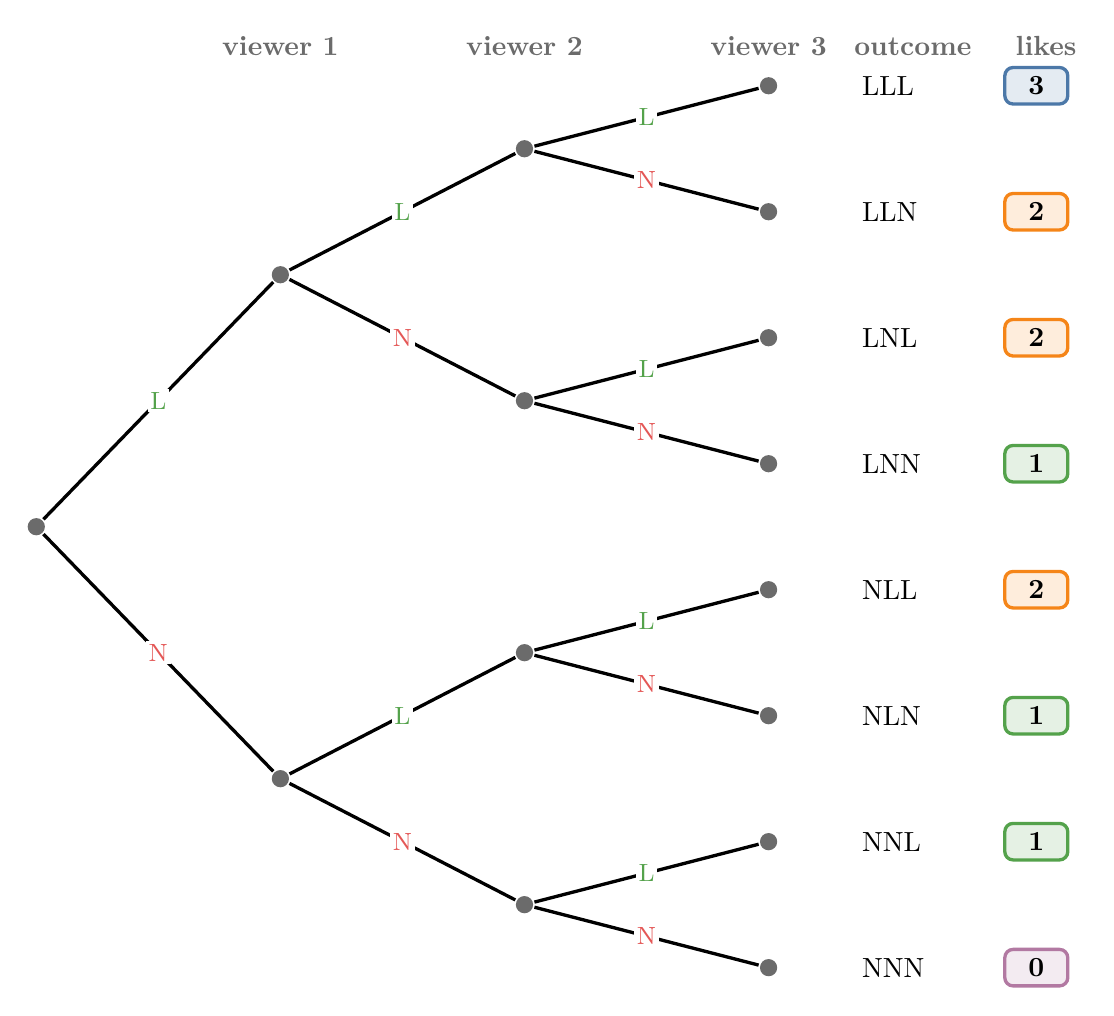
\begin{tikzpicture}[
    grow=right, level distance=3.1cm,
    level 1/.style={sibling distance=6.4cm},
    level 2/.style={sibling distance=3.2cm},
    level 3/.style={sibling distance=1.6cm},
    dot/.style={circle, fill=cgrey, inner sep=2.2pt},
    yes/.style={font=\sffamily\small, text=cgreen, fill=white, inner sep=1pt},
    no/.style={font=\sffamily\small, text=cred, fill=white, inner sep=1pt}]
  \node[dot] (root) {}
    child { node[dot] {}
      child { node[dot] {}
        child { node[dot] (l8) {} edge from parent node[no] {N} }
        child { node[dot] (l7) {} edge from parent node[yes] {L} }
        edge from parent node[no] {N} }
      child { node[dot] {}
        child { node[dot] (l6) {} edge from parent node[no] {N} }
        child { node[dot] (l5) {} edge from parent node[yes] {L} }
        edge from parent node[yes] {L} }
      edge from parent node[no] {N} }
    child { node[dot] {}
      child { node[dot] {}
        child { node[dot] (l4) {} edge from parent node[no] {N} }
        child { node[dot] (l3) {} edge from parent node[yes] {L} }
        edge from parent node[no] {N} }
      child { node[dot] {}
        child { node[dot] (l2) {} edge from parent node[no] {N} }
        child { node[dot] (l1) {} edge from parent node[yes] {L} }
        edge from parent node[yes] {L} }
      edge from parent node[yes] {L} };
  % column titles
  \node[note, font=\sffamily\bfseries] at (3.1,6.1) {viewer 1};
  \node[note, font=\sffamily\bfseries] at (6.2,6.1) {viewer 2};
  \node[note, font=\sffamily\bfseries] at (9.3,6.1) {viewer 3};
  \node[note, font=\sffamily\bfseries, anchor=west] at (10.25,6.1) {outcome};
  \node[note, font=\sffamily\bfseries, anchor=west] at (12.3,6.1) {likes};
  % leaves: outcome and number of likes, coloured by the count
  \foreach \l/\o/\k/\c in {l1/LLL/3/cblue, l2/LLN/2/corange, l3/LNL/2/corange, l4/LNN/1/cgreen,
                           l5/NLL/2/corange, l6/NLN/1/cgreen, l7/NNL/1/cgreen, l8/NNN/0/cpurple} {
    \node[anchor=west, font=\sffamily] at ($(\l)+(1.05,0)$) {\o};
    \node[draw=\c, fill=\c!15, rounded corners=3pt, minimum width=0.8cm, font=\sffamily\bfseries]
      at ($(\l)+(3.4,0)$) {\k};
  }
\end{tikzpicture}
\end{document}
